% Gabarit pandoc des corrigés publiés (brut et guidé). Contenu sans marque ni nom de site.
% Compilation : lualatex (latexmk -lualatex).
% Le Markdown reste la source unique : ne pas éditer ce fichier .tex à la main.
\documentclass[11pt,a4paper]{article}

% --- Moteur, polices (Latin Modern) et langue ---------------------------------
\usepackage{iftex}
\ifLuaTeX\else\errmessage{Ce document se compile avec lualatex}\fi
\usepackage{amsmath,amssymb,mathtools}
\usepackage{fontspec}
% mathrm=sym : \mathrm prend ses glyphes dans la police mathématique (ℓ, μ, Ω), comme KaTeX.
\usepackage[math-style=TeX,bold-style=TeX,mathrm=sym]{unicode-math}
% Repli pour les glyphes absents de Latin Modern (indices et exposants Unicode,
% flèches, filets des schémas en texte, symboles) : DejaVu, puis Latin Modern Math
% (ℓ, lettres mathématiques Unicode des légendes).
\directlua{
  luaotfload.add_fallback("repliTexte", {"DejaVuSerif:mode=harf;", "DejaVuSans:mode=harf;", "file:latinmodern-math.otf:mode=harf;"})
  luaotfload.add_fallback("repliMono", {"DejaVuSansMono:mode=harf;", "DejaVuSans:mode=harf;", "file:latinmodern-math.otf:mode=harf;"})
}
\setmainfont{Latin Modern Roman}[RawFeature={fallback=repliTexte}]
\setsansfont{Latin Modern Sans}[RawFeature={fallback=repliTexte}]
\setmonofont{Latin Modern Mono}[RawFeature={fallback=repliMono}]
\setmathfont{Latin Modern Math}
\usepackage[french]{babel}
\frenchsetup{SmallCapsFigTabCaptions=false}

% --- Mise en page --------------------------------------------------------------
\usepackage[a4paper,margin=2.2cm,headheight=14pt,footskip=1.2cm]{geometry}
\usepackage{microtype}
\setlength{\emergencystretch}{4em}
\tolerance=1500
\setlength{\parindent}{0pt}
\setlength{\parskip}{0.55\baselineskip plus 2pt minus 1pt}
\usepackage{xcolor}
% Gris nommés : babel-french rend « ! » actif dans le document.
\definecolor{gris2}{gray}{0.98}
\definecolor{gris3}{gray}{0.97}
\definecolor{gris5}{gray}{0.95}
\definecolor{gris35}{gray}{0.65}
\definecolor{gris40}{gray}{0.60}
\definecolor{gris45}{gray}{0.55}
\definecolor{gris50}{gray}{0.50}
\definecolor{gris55}{gray}{0.45}
\definecolor{gris60}{gray}{0.40}
\definecolor{gris65}{gray}{0.35}
\definecolor{gris70}{gray}{0.30}
\definecolor{gris80}{gray}{0.20}
\definecolor{gris85}{gray}{0.15}
\usepackage{graphicx}
\usepackage{float}
\usepackage{caption}
\captionsetup{font=small,labelformat=empty,justification=centering}
\usepackage{booktabs,longtable,array,multirow,calc}
\usepackage{siunitx}
\sisetup{locale=FR}
\usepackage[version=4]{mhchem}
\usepackage{listings}
\usepackage{fancyhdr}
\usepackage{lastpage}
\usepackage[most]{tcolorbox}
\usepackage{enumitem}
\setlist{nosep,leftmargin=*,topsep=2pt}
\usepackage[hidelinks,unicode]{hyperref}
\usepackage{bookmark}
\hypersetup{pdftitle={Agro-Véto TB — Algorithmique et informatique 2026},pdfauthor={Rédigé par IA},pdfcreator={LaTeX},pdfsubject={Corrigé brut}}
\usepackage{xurl}

% --- Pandoc : listes, tableaux, figures ----------------------------------------
\providecommand{\passthrough}[1]{#1}
\providecommand{\tightlist}{\setlength{\itemsep}{0pt}\setlength{\parskip}{0pt}}

\makeatletter
\def\maxwidth{\ifdim\Gin@nat@width>\linewidth\linewidth\else\Gin@nat@width\fi}
\def\maxheight{\ifdim\Gin@nat@height>0.55\textheight 0.55\textheight\else\Gin@nat@height\fi}
\makeatother
\setkeys{Gin}{width=\maxwidth,height=\maxheight,keepaspectratio}
\setcounter{secnumdepth}{-\maxdimen}
\providecommand{\pandocbounded}[1]{#1}
\usepackage{longtable,booktabs,array}

% --- Code (listings) -----------------------------------------------------------
\lstset{
  basicstyle=\ttfamily\small,
  columns=fullflexible,
  keepspaces=true,
  breaklines=true,
  breakatwhitespace=false,
  postbreak=\mbox{\textcolor{gris50}{$\hookrightarrow$}\space},
  frame=single,
  rulecolor=\color{gris35},
  framesep=4pt,
  xleftmargin=5pt,xrightmargin=5pt,
  backgroundcolor=\color{gris3},
  keywordstyle=\bfseries,
  commentstyle=\color{gris65},
  stringstyle=\color{gris80},
  showstringspaces=false,
  tabsize=4,
  extendedchars=true,
  aboveskip=6pt,belowskip=6pt,
}

% --- Macros des corrigés (KaTeX ↔ LaTeX) ---------------------------------------
% Les corrigés sont écrits pour KaTeX : on définit ici ce que KaTeX connaît et
% que LaTeX n'a pas, sans jamais retoucher le Markdown.
\providecommand{\R}{\mathbb{R}}
\providecommand{\N}{\mathbb{N}}
\providecommand{\Z}{\mathbb{Z}}
\providecommand{\Q}{\mathbb{Q}}
\providecommand{\C}{\mathbb{C}}
\providecommand{\dd}{\mathrm{d}}
\providecommand{\llbracket}{\lBrack}
\providecommand{\rrbracket}{\rBrack}
\providecommand{\lBrace}{\lbrace}
\providecommand{\rBrace}{\rbrace}
\providecommand{\Box}{\square}
\providecommand{\Diamond}{\lozenge}
\providecommand{\varnothing}{\emptyset}
\providecommand{\argmax}{\operatorname*{arg\,max}}
\providecommand{\argmin}{\operatorname*{arg\,min}}
\renewcommand{\leq}{\leqslant}
\renewcommand{\geq}{\geqslant}

% Équation hors texte : réduite à la largeur de la ligne si elle déborde.
\newsavebox{\boiteequation}
\newcommand{\equationajustee}[1]{%
  \sbox{\boiteequation}{$\displaystyle #1$}%
  \ifdim\wd\boiteequation>\linewidth
    \[\resizebox{\linewidth}{!}{\usebox{\boiteequation}}\]%
  \else
    \[#1\]%
  \fi}

% --- Encadrés pédagogiques (sobres, lisibles en noir et blanc) -----------------
\tcbset{
  encadre/.style={
    enhanced,breakable,sharp corners,
    colback=white,colframe=gris55,
    boxrule=0.4pt,leftrule=2.2pt,
    left=6pt,right=6pt,top=3pt,bottom=3pt,
    before skip=6pt,after skip=6pt,
    fonttitle=\bfseries\small,coltitle=black,
    attach title to upper,after title={\quad},
    parbox=false,
  }
}
\newtcolorbox{indication}[1]{encadre,colframe=gris45,colback=gris2,title={Indication~#1}}
\newtcolorbox{methode}{encadre,colframe=gris70,title={Méthode}}
\newtcolorbox{piege}{encadre,colframe=gris85,boxrule=0.8pt,leftrule=2.2pt,title={Piège}}
\newtcolorbox{jury}{encadre,colframe=gris60,colback=gris5,title={Jury}}
\newtcolorbox{encadrenote}{encadre,colframe=gris40}

% --- Titres de section ---------------------------------------------------------
\usepackage{titlesec}
\titleformat{\section}{\Large\bfseries}{}{0pt}{}
\titleformat{\subsection}{\large\bfseries}{}{0pt}{}
\titleformat{\subsubsection}{\normalsize\bfseries}{}{0pt}{}
\titlespacing*{\section}{0pt}{14pt plus 4pt minus 2pt}{6pt}
\titlespacing*{\subsection}{0pt}{10pt plus 3pt minus 2pt}{4pt}
\titlespacing*{\subsubsection}{0pt}{8pt plus 2pt minus 2pt}{2pt}

% --- En-tête et pied de page ---------------------------------------------------
\pagestyle{fancy}
\fancyhf{}
\fancyhead[L]{\small\textsc{Corrigé brut} · Agro-Véto TB}
\fancyhead[R]{\small Algorithmique et informatique 2026}
\fancyfoot[L]{\footnotesize Corrigé rédigé par IA, non officiel}
\fancyfoot[R]{\footnotesize \thepage\,/\,\pageref*{LastPage}}
\renewcommand{\headrulewidth}{0.4pt}
\renewcommand{\footrulewidth}{0pt}
\fancypagestyle{plain}{\fancyhf{}\fancyfoot[R]{\footnotesize \thepage\,/\,\pageref*{LastPage}}\fancyfoot[L]{\footnotesize Corrigé rédigé par IA, non officiel}\renewcommand{\headrulewidth}{0pt}}

\begin{document}
\thispagestyle{plain}
\begin{center}
  {\small\scshape Corrigé brut}\par\smallskip
  {\LARGE\bfseries Agro-Véto TB — Algorithmique et informatique 2026\par}\medskip
  {\large Agro-Véto · TB · Algorithmique et informatique · 2026\par}
\end{center}
\vspace{2pt}\hrule\vspace{8pt}

\emph{Corrigé rédigé par IA, non officiel. Signalez toute erreur.}

Notations : \texttt{mot1} est de longueur \(n\), \texttt{mot2} de longueur \(p\). Tous les codes sont en Python.

\hypertarget{partie-i-impluxe9mentation-des-opuxe9rations}{%
\section{Partie I --- Implémentation des opérations}\label{partie-i-impluxe9mentation-des-opuxe9rations}}

\hypertarget{question-1-a}{%
\subsection{Question 1 a)}\label{question-1-a}}

Supprimer le caractère d'indice \(i\in[\![0,n-1]\!]\), c'est concaténer le préfixe de longueur \(i\) et le suffixe qui commence juste après ce caractère :

\begin{lstlisting}[language=Python]
def suppression(mot, i):
    return mot[:i] + mot[i+1:]
\end{lstlisting}

Contrôle : \texttt{suppression(\allowbreak{}\textquotesingle{}agro\textquotesingle{},\allowbreak{}0)\allowbreak{}}, \texttt{suppression(\allowbreak{}\textquotesingle{}agro\textquotesingle{},\allowbreak{}2)\allowbreak{}}, \texttt{suppression(\allowbreak{}\textquotesingle{}agro\textquotesingle{},\allowbreak{}3)\allowbreak{}} donnent \texttt{\textquotesingle{}gro\textquotesingle{}}, \texttt{\textquotesingle{}ago\textquotesingle{}}, \texttt{\textquotesingle{}agr\textquotesingle{}}.

\hypertarget{question-1-b}{%
\subsection{Question 1 b)}\label{question-1-b}}

Insérer \texttt{c} à l'indice \(i\in[\![0,n]\!]\), c'est placer \texttt{c} entre le préfixe de longueur \(i\) et le suffixe commençant à l'indice \(i\). Aucun caractère n'est perdu : la longueur passe à \(n+1\).

\begin{lstlisting}[language=Python]
def insertion(mot, i, c):
    return mot[:i] + c + mot[i:]
\end{lstlisting}

Contrôle : avec \texttt{c\ =\ \textquotesingle{}*\textquotesingle{}} et \texttt{mot\ =\ \textquotesingle{}agro\textquotesingle{}}, les indices 0, 2, 4 donnent \texttt{\textquotesingle{}*agro\textquotesingle{}}, \texttt{\textquotesingle{}ag*ro\textquotesingle{}}, \texttt{\textquotesingle{}agro*\textquotesingle{}}.

\begin{figure}[H]
\centering
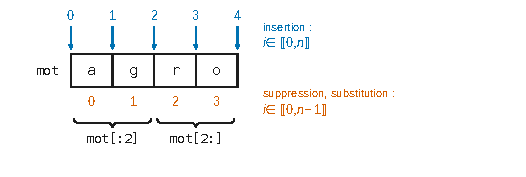
\includegraphics{figures/q1-indices-operations.pdf}
\caption*{Figure 1 --- Indices des opérations sur la chaîne `agro' (n = 4) : n + 1
positions d'insertion entre les caractères, n indices de caractère pour
la suppression et la substitution ; le préfixe `ag' et le suffixe `ro'
se séparent en position 2}
\end{figure}

\hypertarget{partie-ii-ruxe9solution-nauxefve-par-force-brute}{%
\section{Partie II --- Résolution naïve par force brute}\label{partie-ii-ruxe9solution-nauxefve-par-force-brute}}

\hypertarget{question-2}{%
\subsection{Question 2}\label{question-2}}

On n'ajoute un caractère que s'il n'a pas encore été rencontré, c'est-à-dire s'il n'est pas déjà dans \texttt{L} :

\begin{lstlisting}[language=Python]
def lettres(mot):
    L = []
    for car in mot:
        if car not in L:       # ligne 4
            L.append(car)      # ligne 5
    return L
\end{lstlisting}

À chaque tour, \texttt{L} contient sans répétition, dans l'ordre de première apparition, les caractères déjà parcourus. Pour \texttt{\textquotesingle{}concours\textquotesingle{}}, les seconds \texttt{c} et \texttt{o} sont écartés : on obtient \texttt{{[}\textquotesingle{}c\textquotesingle{},\allowbreak{}\textquotesingle{}o\textquotesingle{},\allowbreak{}\textquotesingle{}n\textquotesingle{},\allowbreak{}\textquotesingle{}u\textquotesingle{},\allowbreak{}\textquotesingle{}r\textquotesingle{},\allowbreak{}\textquotesingle{}s\textquotesingle{}{]}\allowbreak{}}.

\hypertarget{question-3}{%
\subsection{Question 3}\label{question-3}}

Notons \(m\) = \texttt{len(mot)}. La boucle \texttt{for\ i\ in\ range(\allowbreak{}len(\allowbreak{}mot)\allowbreak{})\allowbreak{}} décrit les indices \(0\) à \(m-1\) : elle sert aux suppressions (ligne 10, sans caractère), aux substitutions et aux insertions à l'indice \(i\) (lignes 12 et 13, pour chaque caractère de \texttt{mot2}). La boucle de la ligne 14 est hors de la boucle sur \texttt{i} : elle traite la position d'insertion manquante \(m\) (ajout en fin de chaîne).

\begin{lstlisting}[language=Python]
def force_brute(mot1, mot2):
    Dict = {0: [mot1]}
    d = 0
    lettres_mot2 = lettres(mot2)
    while True:
        d += 1
        Dict[d] = []
        for mot in Dict[d-1]:
            for i in range(len(mot)):
                Dict[d].append(suppression(mot, i))                 # ligne 10
                for car in lettres_mot2:
                    Dict[d].append(substitution(mot, i, car))       # ligne 12
                    Dict[d].append(insertion(mot, i, car))          # ligne 13
            for car in lettres_mot2:
                Dict[d].append(insertion(mot, len(mot), car))       # ligne 15
        if mot2 in Dict[d]:
            return d
\end{lstlisting}

(Les lignes 12 et 13 peuvent être échangées.) Ainsi \texttt{Dict{[}d{]}} contient toutes les chaînes obtenues de \texttt{mot1} par \(d\) opérations n'insérant ou ne substituant que des caractères de \texttt{mot2} ; une suite minimale d'opérations peut toujours être choisie ainsi, et toute chaîne de \texttt{Dict{[}d{]}} est à distance au plus \(d\) de \texttt{mot1}. Le premier \(d\) tel que \texttt{mot2} figure dans \texttt{Dict{[}d{]}} est donc la distance d'édition.

\hypertarget{question-4-a}{%
\subsection{Question 4 a)}\label{question-4-a}}

Ici \texttt{lettres(\allowbreak{}\textquotesingle{}AGCTT\textquotesingle{})\allowbreak{}\ =\allowbreak{}\ {[}\textquotesingle{}A\textquotesingle{},\allowbreak{}\textquotesingle{}G\textquotesingle{},\allowbreak{}\textquotesingle{}C\textquotesingle{},\allowbreak{}\textquotesingle{}T\textquotesingle{}{]}\allowbreak{}}, donc \(k=4\) caractères. Pour un mot de longueur \(m\) traité dans la boucle de la ligne 8, les \texttt{append} exécutés sont :

\begin{itemize}
\tightlist
\item
  ligne 10 : \(m\) suppressions (chaînes de longueur \(m-1\)) ;
\item
  ligne 12 : \(km\) substitutions (longueur \(m\)) ;
\item
  ligne 13 : \(km\) insertions avant l'un des caractères (longueur \(m+1\)) ;
\item
  ligne 15 : \(k\) insertions en fin de chaîne (longueur \(m+1\)).
\end{itemize}

Un mot de longueur \(m\) fournit donc \(N(m)\) éléments, les doublons étant comptés (\texttt{append} ajoute sans test) :

\equationajustee{\begin{aligned}
N(m) &= m+2km+k\\
&= 9m+4.
\end{aligned}}

\texttt{Dict{[}0{]}} ne contient que \texttt{\textquotesingle{}ACG\textquotesingle{}}, de longueur 3 :

\equationajustee{\begin{aligned}
|\texttt{Dict[1]}| &= N(3)\\
&= 9\times 3+4
\end{aligned}}

\equationajustee{\boxed{|\texttt{Dict[1]}| = 31}}

\hypertarget{question-4-b}{%
\subsection{Question 4 b)}\label{question-4-b}}

Avec \(m=3\) et \(k=4\) :

\begin{longtable}[]{@{}llll@{}}
\toprule\noalign{}
longueur & 2 (suppressions) & 3 (substitutions) & 4 (insertions) \\
\midrule\noalign{}
\endhead
\bottomrule\noalign{}
\endlastfoot
nombre d'éléments & \(m=3\) & \(km=12\) & \(k(m+1)=16\) \\
\end{longtable}

\textbf{\texttt{Dict{[}1{]}} contient 3 chaînes de longueur 2, 12 de longueur 3 et 16 de longueur 4} (\(3+12+16=31\)).

\hypertarget{question-4-c}{%
\subsection{Question 4 c)}\label{question-4-c}}

\texttt{mot2\ =\ \textquotesingle{}AGCTT\textquotesingle{}} est de longueur 5, donc n'est pas dans \texttt{Dict{[}1{]}} : la boucle continue et \texttt{Dict{[}2{]}} est construit à partir de chacun des 31 éléments de \texttt{Dict{[}1{]}}, doublons compris. Avec \(N(2)=22\), \(N(3)=31\), \(N(4)=40\) :

\equationajustee{\begin{aligned}
|\texttt{Dict[2]}| &= 3\,N(2)+12\,N(3)+16\,N(4)\\
&= 66+372+640
\end{aligned}}

\equationajustee{\boxed{|\texttt{Dict[2]}| = 1078}}

\hypertarget{partie-iii-ruxe9solution-par-programmation-dynamique}{%
\section{Partie III --- Résolution par programmation dynamique}\label{partie-iii-ruxe9solution-par-programmation-dynamique}}

\hypertarget{question-5}{%
\subsection{Question 5}\label{question-5}}

\texttt{mot1\ =\ \textquotesingle{}ACTCT\textquotesingle{}} (\(n=5\)) indexe les lignes, \texttt{mot2\ =\ \textquotesingle{}AGTCAG\textquotesingle{}} (\(p=6\)) les colonnes. La première ligne vaut \(0,\dots,6\) et la première colonne \(0,\dots,5\).

On remplit ensuite ligne par ligne. Si \texttt{mot1{[}i-1{]}\allowbreak{}\ =\allowbreak{}=\allowbreak{}\ mot2{[}j-1{]}\allowbreak{}}, on recopie la case diagonale \(D(i-1,j-1)\). Sinon, on prend 1 plus le minimum des trois voisines (gauche, haut, diagonale).

\begin{figure}[H]
\centering
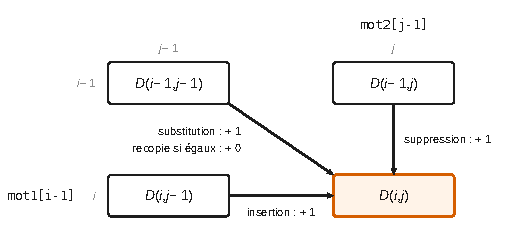
\includegraphics{figures/q5-dependances-case.pdf}
\caption*{Figure 2 --- Les trois cases dont dépend D(i, j) : insertion depuis la
gauche, suppression depuis le haut, substitution depuis la diagonale,
chacune de coût 1 ; recopie gratuite de la diagonale si les deux
caractères comparés sont égaux}
\end{figure}

Cases à égalité de caractères :

\begin{itemize}
\tightlist
\item
  \texttt{A} : cases (1,1) et (1,5) ;
\item
  \texttt{C} : cases (2,4) et (4,4) ;
\item
  \texttt{T} : cases (3,3) et (5,3).
\end{itemize}

Quelques cases :

\begin{longtable}[]{@{}llll@{}}
\toprule\noalign{}
case & caractères & calcul & valeur \\
\midrule\noalign{}
\endhead
\bottomrule\noalign{}
\endlastfoot
(1,5) & \texttt{A} = \texttt{A} & \(D(0,4)\) & 4 \\
(4,4) & \texttt{C} = \texttt{C} & \(D(3,3)\) & 1 \\
(5,3) & \texttt{T} = \texttt{T} & \(D(4,2)\) & 3 \\
(5,6) & \texttt{T} ≠ \texttt{G} & \(1+\min(2,3,2)\) & 3 \\
\end{longtable}

Pour la dernière case, les trois voisines sont \(D(5,5)=2\), \(D(4,6)=3\) et \(D(4,5)=2\).

\begin{longtable}[]{@{}llllllll@{}}
\toprule\noalign{}
& & A & G & T & C & A & G \\
\midrule\noalign{}
\endhead
\bottomrule\noalign{}
\endlastfoot
& \textbf{0} & 1 & 2 & 3 & 4 & 5 & 6 \\
\textbf{A} & 1 & 0 & 1 & 2 & 3 & 4 & 5 \\
\textbf{C} & 2 & 1 & 1 & 2 & 2 & 3 & 4 \\
\textbf{T} & 3 & 2 & 2 & 1 & 2 & 3 & 4 \\
\textbf{C} & 4 & 3 & 3 & 2 & 1 & 2 & 3 \\
\textbf{T} & 5 & 4 & 4 & 3 & 2 & 2 & \textbf{3} \\
\end{longtable}

\equationajustee{\boxed{D(5,6)=3}}

\hypertarget{question-6}{%
\subsection{Question 6}\label{question-6}}

\textbf{Les fonctions \texttt{matrice\_nulle\_1} et \texttt{matrice\_nulle\_4}.}

(La fonction 2 crée \(n+1\) références vers une même liste : modifier une case modifie toute la colonne. La fonction 3 crée \(p+1\) lignes de \(n+1\) éléments, c'est-à-dire la transposée.)

\begin{figure}[H]
\centering
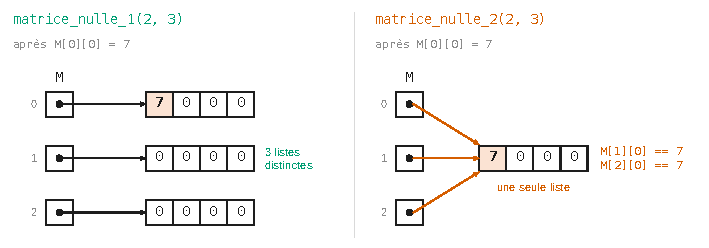
\includegraphics{figures/q6-alias-matrice-nulle.pdf}
\caption*{Figure 3 --- Listes en mémoire pour n = 2 et p = 3, après avoir mis 7
dans la case (0, 0) : matrice\_nulle\_1 crée trois listes distinctes,
matrice\_nulle\_2 trois références vers une même liste, dont toute la
colonne 0 vaut alors 7}
\end{figure}

\hypertarget{question-7}{%
\subsection{Question 7}\label{question-7}}

\begin{lstlisting}[language=Python]
def matrice_levenshtein(mot1, mot2):
    n, p = len(mot1), len(mot2)
    D = matrice_nulle(n, p)                                         # ligne 3
    for j in range(p+1):
        D[0][j] = j                                                 # ligne 5
    for i in range(n+1):
        D[i][0] = i                                                 # ligne 7
    for i in range(1, n+1):
        for j in range(1, p+1):
            if mot1[i-1] == mot2[j-1]:
                D[i][j] = D[i-1][j-1]                               # ligne 11
            else:
                D[i][j] = 1 + min(D[i][j-1], D[i-1][j], D[i-1][j-1])  # ligne 13
    return D
\end{lstlisting}

Le parcours par lignes puis colonnes croissantes garantit que les trois cases voisines (gauche, haut, diagonale) sont déjà calculées lorsqu'on calcule \(D(i,j)\). Coût en temps et en mémoire : \(O(np)\).

\hypertarget{question-8}{%
\subsection{Question 8}\label{question-8}}

D'après l'énoncé, la distance d'édition de \texttt{mot1} à \texttt{mot2} est \(D(n,p)\), case en bas à droite de la matrice :

\begin{lstlisting}[language=Python]
def distance(mot1, mot2):
    D = matrice_levenshtein(mot1, mot2)
    return D[len(mot1)][len(mot2)]
\end{lstlisting}

Ainsi \texttt{distance(\allowbreak{}\textquotesingle{}ACT\textquotesingle{},\allowbreak{}\textquotesingle{}AGTC\textquotesingle{})\allowbreak{}} vaut 2 et \texttt{distance(\allowbreak{}\textquotesingle{}ACTCT\textquotesingle{},\allowbreak{}\textquotesingle{}AGTCAG\textquotesingle{})\allowbreak{}} vaut 3.

\hypertarget{partie-iv-application-correcteur-orthographique}{%
\section{Partie IV --- Application : correcteur orthographique}\label{partie-iv-application-correcteur-orthographique}}

\hypertarget{question-9}{%
\subsection{Question 9}\label{question-9}}

\begin{lstlisting}[language=Python]
def correcteur_orthographique(mot):
    n = len(mot)
    dmin = n+1
    M = []
    for chaine in Mots_Francais:
        d = distance(mot, chaine)       # ligne 6
        if d < dmin:
            dmin = d
            M = [chaine]                # ligne 9
        elif d == dmin:
            M.append(chaine)            # ligne 11
    return M
\end{lstlisting}

Invariant : après chaque tour, \texttt{dmin} est la plus petite distance de \texttt{mot} aux mots déjà examinés et \texttt{M} la liste de ces mots réalisant \texttt{dmin}. Un mot strictement plus proche invalide les précédents (ligne 9 : on repart d'une liste à un élément) ; un mot à égalité s'ajoute (ligne 11). L'initialisation \texttt{dmin\ =\ n+1} convient : le mot \texttt{\textquotesingle{}a\textquotesingle{}} est à distance au plus \(\max(n,1)\le n+1\) de \texttt{mot}, donc \texttt{M} n'est jamais vide en fin de parcours.

\hypertarget{partie-v-obtention-dune-suite-dopuxe9rations-minimale}{%
\section{Partie V --- Obtention d'une suite d'opérations minimale}\label{partie-v-obtention-dune-suite-dopuxe9rations-minimale}}

\hypertarget{question-10}{%
\subsection{Question 10}\label{question-10}}

On remonte depuis la case (5,6) de la matrice de la question 5, avec la chaîne courante \(\texttt{mot}(i,j)\). À chaque étape, on vérifie l'invariant :

\equationajustee{\texttt{mot}(i,j)=\texttt{mot2[:j]}+\texttt{mot1[i:]}}

Le tableau donne, pour chaque case visitée, la valeur des trois voisines ; une voisine est retenue (« oui ») si elle vaut \(D(i,j)-1\). Aux cases d'égalité, la méthode impose la diagonale sans opération.

\begin{longtable}[]{@{}
  >{\raggedright\arraybackslash}p{(\columnwidth - 14\tabcolsep) * \real{0.0886}}
  >{\raggedright\arraybackslash}p{(\columnwidth - 14\tabcolsep) * \real{0.0687}}
  >{\raggedright\arraybackslash}p{(\columnwidth - 14\tabcolsep) * \real{0.1535}}
  >{\raggedright\arraybackslash}p{(\columnwidth - 14\tabcolsep) * \real{0.1254}}
  >{\raggedright\arraybackslash}p{(\columnwidth - 14\tabcolsep) * \real{0.1189}}
  >{\raggedright\arraybackslash}p{(\columnwidth - 14\tabcolsep) * \real{0.0971}}
  >{\raggedright\arraybackslash}p{(\columnwidth - 14\tabcolsep) * \real{0.0971}}
  >{\raggedright\arraybackslash}p{(\columnwidth - 14\tabcolsep) * \real{0.2207}}@{}}
\toprule\noalign{}
\begin{minipage}[b]{\linewidth}\raggedright
case
\end{minipage} & \begin{minipage}[b]{\linewidth}\raggedright
\(D\)
\end{minipage} & \begin{minipage}[b]{\linewidth}\raggedright
chaîne courante
\end{minipage} & \begin{minipage}[b]{\linewidth}\raggedright
caractères
\end{minipage} & \begin{minipage}[b]{\linewidth}\raggedright
diagonale
\end{minipage} & \begin{minipage}[b]{\linewidth}\raggedright
gauche
\end{minipage} & \begin{minipage}[b]{\linewidth}\raggedright
haut
\end{minipage} & \begin{minipage}[b]{\linewidth}\raggedright
pas effectué
\end{minipage} \\
\midrule\noalign{}
\endhead
\bottomrule\noalign{}
\endlastfoot
(5,6) & 3 & \texttt{AGTCAG} & \texttt{T} ≠ \texttt{G} & 2, oui & 2, oui & 3, non & deux branches \\
(4,5) & 2 & \texttt{AGTCAT} & \texttt{C} ≠ \texttt{A} & 2, non & 1, oui & 3, non & suppression de l'indice 4 \\
(5,5) & 2 & \texttt{AGTCA} & \texttt{T} ≠ \texttt{A} & 1, oui & 2, non & 2, non & substitution de l'indice 4 par \texttt{T} \\
(4,4) & 1 & \texttt{AGTCT} & \texttt{C} = \texttt{C} & & & & diagonale, sans opération \\
(3,3) & 1 & \texttt{AGTCT} & \texttt{T} = \texttt{T} & & & & diagonale, sans opération \\
(2,2) & 1 & \texttt{AGTCT} & \texttt{C} ≠ \texttt{G} & 0, oui & 1, non & 1, non & substitution de l'indice 1 par \texttt{C} \\
(1,1) & 0 & \texttt{ACTCT} & \texttt{A} = \texttt{A} & & & & diagonale vers (0,0) \\
\end{longtable}

\begin{itemize}
\tightlist
\item
  \textbf{Branche 1} : en (5,6), substitution à l'indice 5 par \texttt{mot1{[}4{]}\ =\ \textquotesingle{}T\textquotesingle{}}, d'où \texttt{AGTCAT} en (4,5) ; puis suppression de l'indice 4, d'où \texttt{AGTCT} en (4,4).
\item
  \textbf{Branche 2} : en (5,6), suppression de l'indice 5, d'où \texttt{AGTCA} en (5,5) ; puis substitution de l'indice 4 par \texttt{mot1{[}4{]}\ =\ \textquotesingle{}T\textquotesingle{}}, d'où \texttt{AGTCT} en (4,4).
\item
  \textbf{Partie commune} depuis (4,4) : deux remontées diagonales sans opération, puis en (2,2) substitution de l'indice 1 par \texttt{mot1{[}1{]}\ =\ \textquotesingle{}C\textquotesingle{}}, d'où \texttt{ACTCT} en (1,1), et une dernière diagonale vers (0,0).
\end{itemize}

Il y a donc \textbf{exactement deux suites minimales} (3 opérations chacune, conformément à \(D(5,6)=3\)) :

\equationajustee{\boxed{\begin{aligned}{}&\texttt{ACTCT}\longrightarrow\texttt{AGTCT}\longrightarrow\texttt{AGTCAT}\longrightarrow\texttt{AGTCAG}\\
&\texttt{ACTCT}\longrightarrow\texttt{AGTCT}\longrightarrow\texttt{AGTCA}\longrightarrow\texttt{AGTCAG}
\end{aligned}}}

Lues dans le sens direct : la première substitue \texttt{C}→\texttt{G} à l'indice 1, insère \texttt{A} à l'indice 4, substitue \texttt{T}→\texttt{G} à l'indice 5 ; la seconde substitue \texttt{C}→\texttt{G} à l'indice 1, substitue \texttt{T}→\texttt{A} à l'indice 4, insère \texttt{G} à l'indice 5.

\begin{figure}[H]
\centering
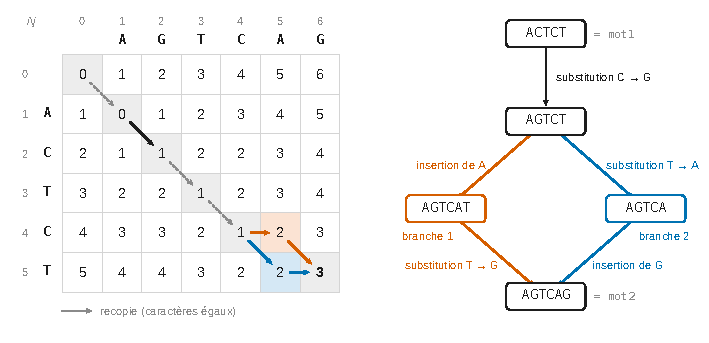
\includegraphics{figures/q10-chemins-matrice.pdf}
\caption*{Figure 4 --- Les deux chemins optimaux dans la matrice D de la question
5, orientés de (0,0) vers (5,6) (la remontée les parcourt à l'envers),
et les deux suites minimales de 3 opérations de ACTCT à AGTCAG}
\end{figure}

\hypertarget{question-11}{%
\subsection{Question 11}\label{question-11}}

On applique à \texttt{mot} les opérations décrites dans la partie V avec les fonctions de la partie I :

\begin{lstlisting}[language=Python]
def suite_operations(mot1, mot2):
    D = matrice_levenshtein(mot1, mot2)                 # ligne 2
    Suite_chgt = [mot2]
    mot = mot2
    i, j = len(mot1), len(mot2)
    while i > 0 or j > 0:
        if i>0 and j>0 and mot1[i-1] == mot2[j-1]:
            i, j = i-1, j-1
        elif i>0 and j>0 and D[i-1][j-1] == D[i][j]-1:
            mot = substitution(mot, j-1, mot1[i-1])     # ligne 10
            i, j = i-1, j-1
            Suite_chgt = [mot] + Suite_chgt
        elif j > 0 and D[i][j-1] == D[i][j] -1:
            mot = suppression(mot, j-1)                 # ligne 14
            j = j-1
            Suite_chgt = [mot] + Suite_chgt
        elif i > 0 and D[i-1][j] == D[i][j]-1:
            mot = insertion(mot, j, mot1[i-1])          # ligne 18
            Suite_chgt = [mot] + Suite_chgt
            i = i-1
    return Suite_chgt
\end{lstlisting}

Invariant en entrée de chaque tour :

\equationajustee{\texttt{mot}=\texttt{mot2[:j]}+\texttt{mot1[i:]}}

Chacune des trois opérations le rétablit pour la nouvelle case ; en (0,0), \texttt{mot} vaut donc \texttt{mot1}.

La boucle termine car \(i+j\) décroît strictement. Elle ne se bloque jamais : hors des bords, la relation de récurrence garantit qu'une voisine vaut \(D(i,j)-1\) ; sur les bords, les valeurs initiales \(D(0,j)=j\) et \(D(i,0)=i\) le garantissent aussi.

La liste renvoyée contient \(D(n,p)+1\) chaînes : la suite est minimale. Sur l'exemple de la question 10, la fonction renvoie \texttt{{[}\textquotesingle{}ACTCT\textquotesingle{},\allowbreak{}\ \textquotesingle{}AGTCT\textquotesingle{},\allowbreak{}\ \textquotesingle{}AGTCAT\textquotesingle{},\allowbreak{}\ \textquotesingle{}AGTCAG\textquotesingle{}{]}\allowbreak{}} (la diagonale est testée avant la gauche).

\end{document}
